% =============================================================================
%  HW03 REPORT — Preferencias de sushi en Japón: un análisis de elección discreta
%  Curso: Understanding Consumer Behavior Through Discrete Choice Models
%  Universidad de Concepción, Depto. Ingeniería Industrial
%  Compilar: pdflatex x2 (ver compile.bat)
% =============================================================================
\documentclass[12pt,a4paper]{article}

% --- packages ---
\usepackage[utf8]{inputenc}
\usepackage[T1]{fontenc}
\usepackage[spanish,es-tabla]{babel}
\usepackage{lmodern}
\usepackage[margin=2.5cm]{geometry}
\usepackage{amsmath,amssymb}
\usepackage{booktabs}
\usepackage{graphicx}
\usepackage{hyperref}
\usepackage{caption}
\usepackage{subcaption}
\usepackage{float}
\usepackage{enumitem}
\usepackage{multirow}
\usepackage{array}
\usepackage[table]{xcolor}

\hypersetup{
  colorlinks=true,
  linkcolor=blue!60!black,
  citecolor=blue!40!black,
  urlcolor=blue!60!black,
}

% --- paths ---
\graphicspath{{figures/}{Imagenes/}}

% absorbe overfull menores estirando el espaciado en vez de salirse del margen
\emergencystretch=3em

\begin{document}

% =============================================================================
% PORTADA (formato Tarea 1)
% =============================================================================
\begin{titlepage}
  \centering
  
\includegraphics[width=0.5\textwidth]{logo_dii.png}\\[2cm]

  {\Large\bfseries Homework Assignment No.~3}\\[12pt]
  {\LARGE\bfseries Preferencias de sushi en Japón: un análisis de elección discreta de la heterogeneidad del consumidor}\\[8pt]

  {\large Understanding Consumer Behavior through Discrete Choice Models}\\[4pt]
  {\large 2026--1}\\[2.5cm]

  {\large Realizado por:}\\[4pt]
  {\large
    \begin{tabular}{l c l}
      Matías Arriagada R. & 2022445068 & \href{mailto:matiaarriagada2022@udec.cl}{matiaarriagada2022@udec.cl} \\[4pt]
      Vicente Soñez I.    & 2022451971 & \href{mailto:vsonez2022@udec.cl}{vsonez2022@udec.cl}
    \end{tabular}
  }\\[2cm]

  {\large Profesor:}\\[4pt]
  {\large Ph.\,D. Sebastián Astroza Tagle}\\[2.5cm]

  \vfill
  {\large 6 de julio de 2026, Concepción, Chile}
\end{titlepage}

\tableofcontents
\newpage

% =============================================================================
\section{Introducción}
% =============================================================================

Comprender el comportamiento del consumidor en el sector alimentario es clave para detectar oportunidades insatisfechas. Aunque en el contexto chileno el sushi ha alcanzado una alta popularidad bajo un formato de comida rápida, esta propuesta dista considerablemente de la gastronomía original japonesa, existiendo una brecha en la oferta de sushi de alta gama. En este sentido, modelar las decisiones de los consumidores en un mercado maduro como el japonés permite extraer lecciones estratégicas para el mercado chileno. Así, el presente estudio busca identificar patrones de preferencia que faciliten el desarrollo de un 'océano azul' en el segmento premium nacional.
\\

Para este propósito se utiliza el 'Sushi Preference Dataset', recopilado por Toshihiro Kamishima (2003) mediante encuestas estructuradas a 5.000 consumidores en Japón. La base de datos se organiza en formato largo, totalizando 50.000 observaciones donde cada registro representa la evaluación de un consumidor frente a una de las 10 alternativas de sushi disponibles. En cada observación, la variable dependiente toma el valor de uno si la alternativa fue seleccionada como la opción preferida (rango 1) y cero en caso contrario, vinculando esta decisión tanto a los atributos del producto (precio, grasa y popularidad) como al perfil demográfico del decisor.

\begin{itemize}[nosep]
  \item \textbf{Set A}: 10 tipos de sushi ordenados por los 5.000 usuarios de más a menos preferido. Los ítems son \texttt{ebi} (camarón), \texttt{anago} (anguila de mar), \texttt{maguro} (atún), \texttt{ika} (calamar), \texttt{uni} (erizo), \texttt{ikura} (huevas de salmón), \texttt{tamago} (huevo), \texttt{toro} (atún graso), \texttt{tekka\_maki} (rollo de atún) y \texttt{kappa\_maki} (rollo de pepino).
  \item \textbf{Demografía}: género, grupo etario, región de residencia (12 regiones, colapsadas a Japón Oriental/Occidental) e indicador de migración.
\end{itemize}

Este informe trabaja exclusivamente sobre el Set A (los 10 ítems que todos los usuarios evalúan), y se organiza en torno a las cuatro secciones exigidas por la pauta: (A)~especificación y estimación, (B)~interpretación de parámetros, (C)~análisis de escenarios y (D)~recomendaciones. Todo el código (Python + R/Apollo) se entrega como pipeline reproducible en una carpeta compartida (ver Linkografía).

% =============================================================================
\section{Model Specification and Estimation (Sección A)}
\label{sec:A}
% =============================================================================

El análisis se articula en torno a \textbf{tres modelos protagonistas}, cada uno respondiendo a una pregunta conductual distinta:

\begin{enumerate}[nosep]
  \item \textbf{M1 --- MNL con ASCs e interacciones demográficas (modelo preferido):} recoge la heterogeneidad observada entre individuos mediante interacciones entre atributos y demografía, identificables junto a constantes específicas por alternativa. Es la base para interpretar el efecto de la edad y la región sobre la preferencia por grasa y precio.
  \item \textbf{M2 --- Nested Logit sobre el ranking explotado:} relaja el supuesto IIA y cuantifica la sustitución observada entre ítems cuando el favorito no está disponible. Soporta el escenario contrafactual de oferta (shock de precio del toro).
  \item \textbf{M3 --- Latent Class MNL:} especificación avanzada con variables latentes; segmenta el mercado en tres tipos de consumidor no observables, identificados a partir del panel de tres pseudo-elecciones por usuario. Es el puente directo entre los hallazgos de M1 y M2 y las recomendaciones de segmentación.
\end{enumerate}

Como apoyo a la justificación estadística se estiman tres modelos \emph{baseline} sin rol interpretativo propio: \textbf{MNL-atributos} (MNL de atributos puros), \textbf{MNL-ASC} (MNL de ASCs puros) y \textbf{MNL-explotado} (MNL de ASCs sobre los datos explotados). Sirven de referencia anidada para los tests de razón de verosimilitud (LR); sus log-verosimilitudes se incluyen en la Tabla~\ref{tab:comparison}.

La utilidad determinista $V_{nj}$ de cada alternativa $j \in \{0, \dots, 9\}$ para el consumidor $n$ sigue la forma MNL estándar con perturbación i.i.d.\ Valor Extremo Tipo I; las especificaciones particulares se detallan en cada subsección.

\subsection{Datos}

Este dataset es real: fue extraído de un paper académico que investigaba las preferencias de consumo de sushi en Japón, y fue actualizado en 2016. El procesamiento convirtió las respuestas de ranking en un modelo de elección única (se toma como elegido el ítem en el primer lugar del ranking de cada usuario) y transformó los archivos originales IDATA/UDATA a formato \texttt{.csv}; todo queda documentado en el repositorio adjunto al final de este informe.

Cada ítem del Set A tiene tres atributos continuos: \texttt{price\_norm} $[1{,}02$--$4{,}49]$, \texttt{oiliness} $[0{,}27$--$3{,}45$; recodificada para que mayor $=$ más grasoso$]$ y \texttt{freq\_sold} $[0{,}40$--$0{,}92]$. Los atributos categóricos (\texttt{style}: maki/otro; \texttt{major\_group}: pescado-marisco/otro) se usan para definir los nidos del Nested Logit. Los shares de primera preferencia observados se muestran en la Figura~\ref{fig:shares}.

\begin{figure}[H]
  \centering
  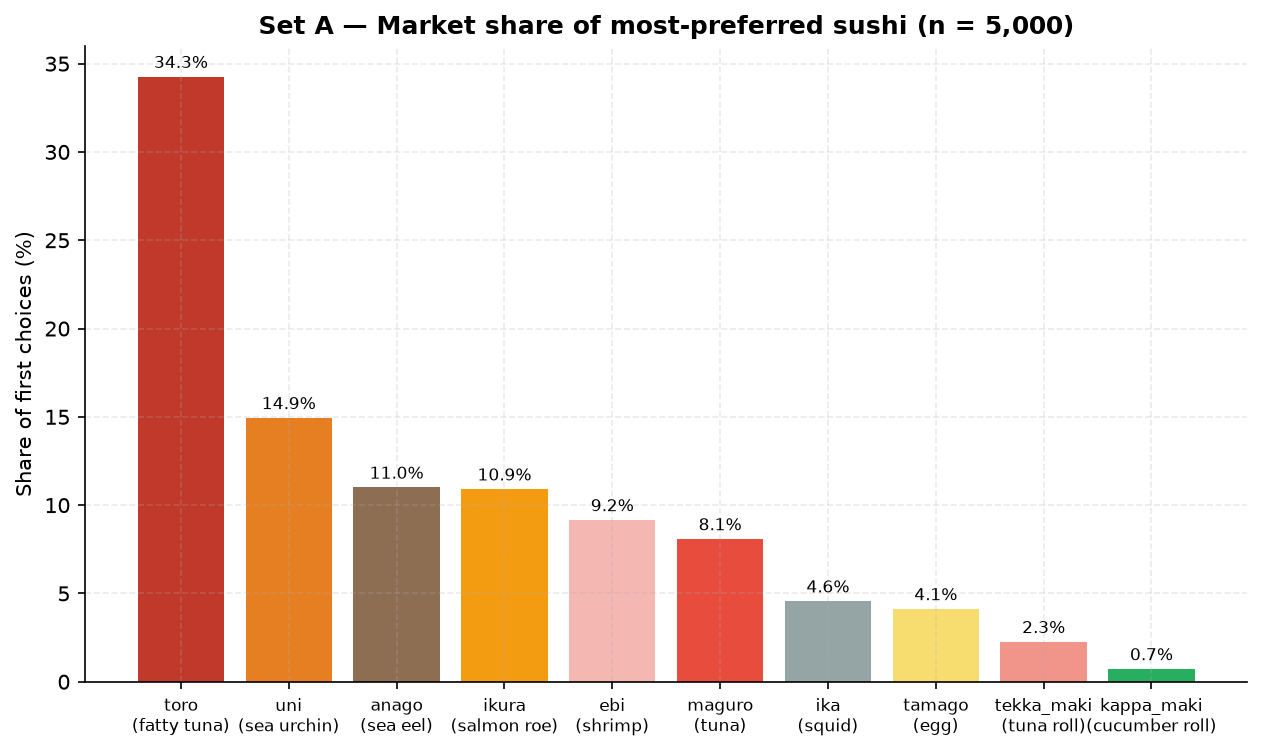
\includegraphics[width=0.72\textwidth]{choice_shares_setA.png}
  \caption{Shares de primera preferencia observados, Set A ($N = 5.000$). Toro domina con 34,3\%, seguido de uni (14,9\%) y anago (11,0\%).}
  \label{fig:shares}
\end{figure}

\begin{figure}[H]
  \centering
  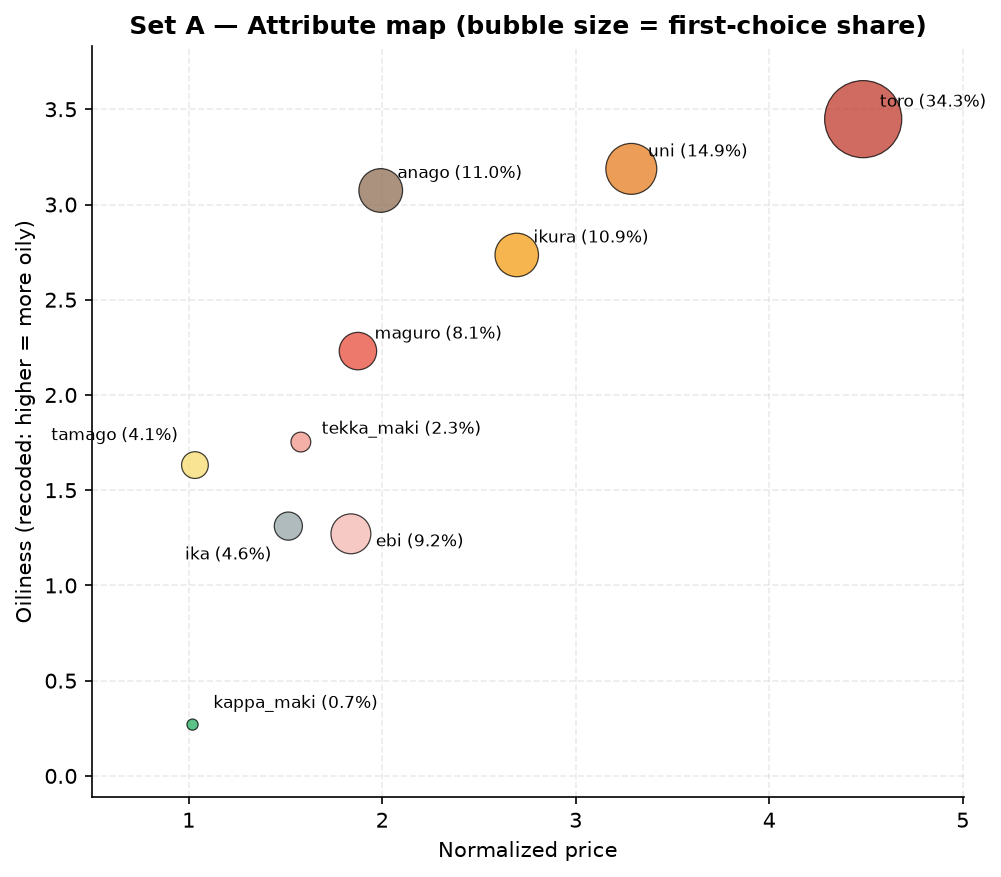
\includegraphics[width=0.62\textwidth]{item_attribute_map.png}
  \caption{Espacio de atributos del Set A: precio vs.\ oiliness, con tamaño de burbuja proporcional al share. Nótese la fuerte asociación entre grasa y popularidad: toro, uni y anago forman el cluster superior derecho.}
  \label{fig:attr_map}
\end{figure}

\subsection{Estrategia de identificación}
\label{sec:ident}

Una propiedad crítica del diseño del Set A es que los tres atributos continuos (\texttt{price\_norm}, \texttt{oiliness}, \texttt{freq\_sold}) son \emph{constantes por ítem}: los 5.000 usuarios ven vectores de atributos idénticos. Con 10 alternativas existen a lo más 9 parámetros independientes de variación entre alternativas, de modo que una especificación con ASCs completos (9 constantes) y betas genéricos de atributos simultáneos sería perfectamente colineal e inestimable. Esto no es un error de datos sino una propiedad del diseño.

El informe lo maneja sin combinar nunca ASCs completos con betas de atributos en la misma especificación. La cadena anidada de baseline
\[
\text{MNL-atributos (3 betas)} \;\subset\; \text{MNL-ASC (9 ASCs)} \;\subset\; \text{M1 (9 ASCs + 3 interacciones)}
\]
permite tests de razón de verosimilitud (LR) limpios en cada eslabón, reportados en la Tabla~\ref{tab:comparison}. Las interacciones demográficas (p.\,ej.\ $\text{oiliness}_j \times \text{edad}_n$) sí son identificables junto a ASCs completos porque varían entre individuos.

\textbf{Constantes calibradas para los escenarios (Train, 2009).} Los escenarios contrafactuales que requieren un coeficiente de atributo (p.\,ej.\ el shock de precio del toro) combinan constantes $C_j$ calibradas para reproducir exactamente los shares observados con los betas de atributo del modelo \textbf{MNL-atributos}. Este enfoque de betas + constantes calibradas es estándar en la literatura (Train, 2009). Cabe una advertencia importante: dentro del Set A $\text{corr}(\text{precio}, \text{oiliness}) = 0{,}82$ (Figura~\ref{fig:corr}), una multicolinealidad severa con sólo 10 ítems que infla los errores estándar de los betas de atributo. En consecuencia, los escenarios de precio se interpretan \emph{cualitativamente} (dirección del efecto y ranking de sustitución), no como magnitudes exactas.

\begin{figure}[H]
  \centering
  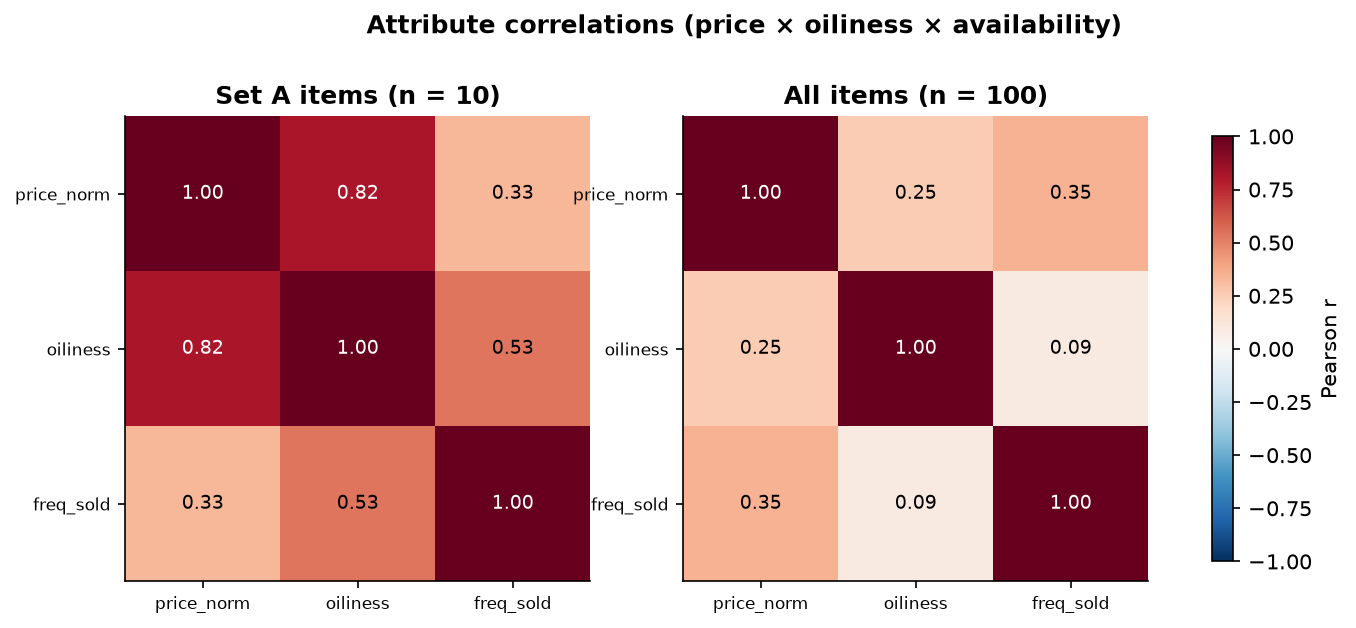
\includegraphics[width=0.5\textwidth]{attribute_correlation.png}
  \caption{Matriz de correlación de los tres atributos continuos en el Set A ($n = 10$ ítems). $\rho(\text{precio}, \text{oiliness}) = 0{,}82$: toro es a la vez el ítem más grasoso y el más caro.}
  \label{fig:corr}
\end{figure}

\subsection{Modelos baseline (referencia para los tests LR)}

Los baseline MNL-atributos (MNL con sólo los tres atributos continuos) y MNL-ASC (MNL con sólo ASCs) no se desarrollan como modelos de interpretación: su rol es servir de referencia anidada para justificar estadísticamente la selección de M1. La cadena MNL-atributos $\subset$ MNL-ASC $\subset$ M1 entrega dos tests LR sucesivos (Tabla~\ref{tab:comparison}):
\begin{itemize}[nosep]
  \item \textbf{LR(MNL-atributos vs.\ MNL-ASC) = 191,3} (gl = 6, $p < 10^{-3}$): los tres atributos observables no capturan toda la heterogeneidad entre ítems; existe calidad no observada sustancial (prestigio, complejidad de sabor, asociaciones culturales) que los ASCs sí recogen. Una regresión OLS descriptiva de los 9 ASCs sobre los 3 atributos entrega $R^2 = 0{,}95$.
  \item \textbf{LR(MNL-ASC vs.\ M1) = 43,7} (gl = 3, $p = 1{,}7 \times 10^{-9}$): la heterogeneidad demográfica es real y significativa, justificando las interacciones de M1.
\end{itemize}
El baseline MNL-atributos cumple además un rol operativo: aporta los coeficientes de precio ($+0{,}581$, $z = 24{,}1$), grasa y disponibilidad que alimentan los escenarios de la Sección~\ref{sec:C} y los trade-offs del Apéndice~\ref{app:wtp}.

\subsection{M1 --- MNL con ASCs + interacciones demográficas (modelo preferido)}

M1 extiende el baseline MNL-ASC con tres interacciones demográficas, que varían entre individuos y por tanto son identificables junto a los ASCs completos:

\begin{equation}
\begin{split}
  U_{nj} = \text{ASC}_j
  &+ \beta_{\text{precio}\times\text{oeste}} \cdot \text{price}_j \cdot \text{oeste}_n \\
  &+ \beta_{\text{oil}\times\text{edad}} \cdot \text{oiliness}_j \cdot \text{edad}_n
   + \beta_{\text{oil}\times\text{oeste}} \cdot \text{oiliness}_j \cdot \text{oeste}_n
   + \varepsilon_{nj}
\end{split}
\label{eq:m1}
\end{equation}

donde $\text{oeste}_n = 1$ si la región actual del encuestado está en Japón Occidental y $\text{edad}_n$ es el grupo etario (0--5, tratado como lineal).

\begin{table}[H]
  \centering
  \small
  \caption{M1 --- MNL con ASCs e interacciones demográficas ($K = 12$)}
  \label{tab:m1}
  \begin{tabular}{lrrrrr}
    \toprule
    Parámetro & Coef. & EE & $z$ & $p$ & IC 95\% \\
    \midrule
    \multicolumn{6}{l}{\textit{Constantes específicas (ref.: ebi)}} \\
    ASC$_{\text{anago}}$      & $-$0,084 & 0,094 & $-$0,90 & 0,369 & [$-$0,267; 0,099] \\
    ASC$_{\text{maguro}}$     & $-$0,265 & 0,077 & $-$3,42 & 0,001 & [$-$0,416; $-$0,113] \\
    ASC$_{\text{ika}}$        & $-$0,711 & 0,081 & $-$8,75 & $< 10^{-3}$ & [$-$0,870; $-$0,551] \\
    ASC$_{\text{uni}}$        &  0,231 & 0,090 &  2,57  & 0,010 & [0,055; 0,406] \\
    ASC$_{\text{ikura}}$      & $-$0,025 & 0,082 & $-$0,31 & 0,758 & [$-$0,185; 0,135] \\
    ASC$_{\text{tamago}}$     & $-$0,869 & 0,087 & $-$10,00& $< 10^{-3}$ & [$-$1,040; $-$0,699] \\
    ASC$_{\text{toro}}$       &  1,041 & 0,092 & 11,32  & $< 10^{-3}$ & [0,861; 1,221] \\
    ASC$_{\text{tekka\_maki}}$& $-$1,475 & 0,107 & $-$13,78& $< 10^{-3}$ & [$-$1,684; $-$1,265] \\
    ASC$_{\text{kappa\_maki}}$& $-$2,426 & 0,176 & $-$13,78& $< 10^{-3}$ & [$-$2,771; $-$2,081] \\
    \addlinespace
    \multicolumn{6}{l}{\textit{Interacciones demográficas}} \\
    $\beta_{\text{precio}\times\text{oeste}}$ & $-$0,066 & 0,045 & $-$1,46 & 0,143 & [$-$0,155; 0,022] \\
    $\beta_{\text{oil}\times\text{edad}}$    & \textbf{0,089} & \textbf{0,017} & \textbf{5,20} & $\mathbf{< 10^{-3}}$ & [0,055; 0,123] \\
    $\beta_{\text{oil}\times\text{oeste}}$   & $-$0,058 & 0,067 & $-$0,86 & 0,389 & [$-$0,189; 0,074] \\
    \bottomrule
    \addlinespace
    \multicolumn{6}{l}{\footnotesize LL = $-$9.733,21\;\; $\rho^2 = 0{,}155$\;\; AIC = 19.490,4\;\; $N = 5.000$} \\
  \end{tabular}
\end{table}

\textbf{Test LR MNL-ASC vs.\ M1}: $\text{LR} = 43{,}7$, $\text{gl} = 3$, $p = 1{,}7 \times 10^{-9}$. La heterogeneidad demográfica es significativa y M1 se prefiere sobre el baseline de ASCs para interpretación conductual.\\[4pt]
\textbf{Robustez (M1r)}: eliminando las dos interacciones con Oeste (ambas de $|z| < 1{,}96$) el LR conjunto contra M1 es $15{,}6$ (gl = 2, $p = 4{,}1 \times 10^{-4}$): son individualmente no significativas pero conjuntamente sí lo son; se retiene la especificación completa M1.

\subsection{M2 --- Nested Logit sobre ranking explotado}
\label{sec:m2}

Para relajar el supuesto IIA e investigar patrones de sustitución, se estima un Nested Logit sobre el \emph{ranking explotado} (ranks 1--3 por usuario). Cada usuario genera tres pseudo-elecciones con choice sets decrecientes (10, 9 y 8 alternativas), aportando 15.000 pseudo-observaciones que contienen la información de sustitución observada (Beggs, Cardell y Hausman, 1981).

\begin{figure}[H]
  \centering
  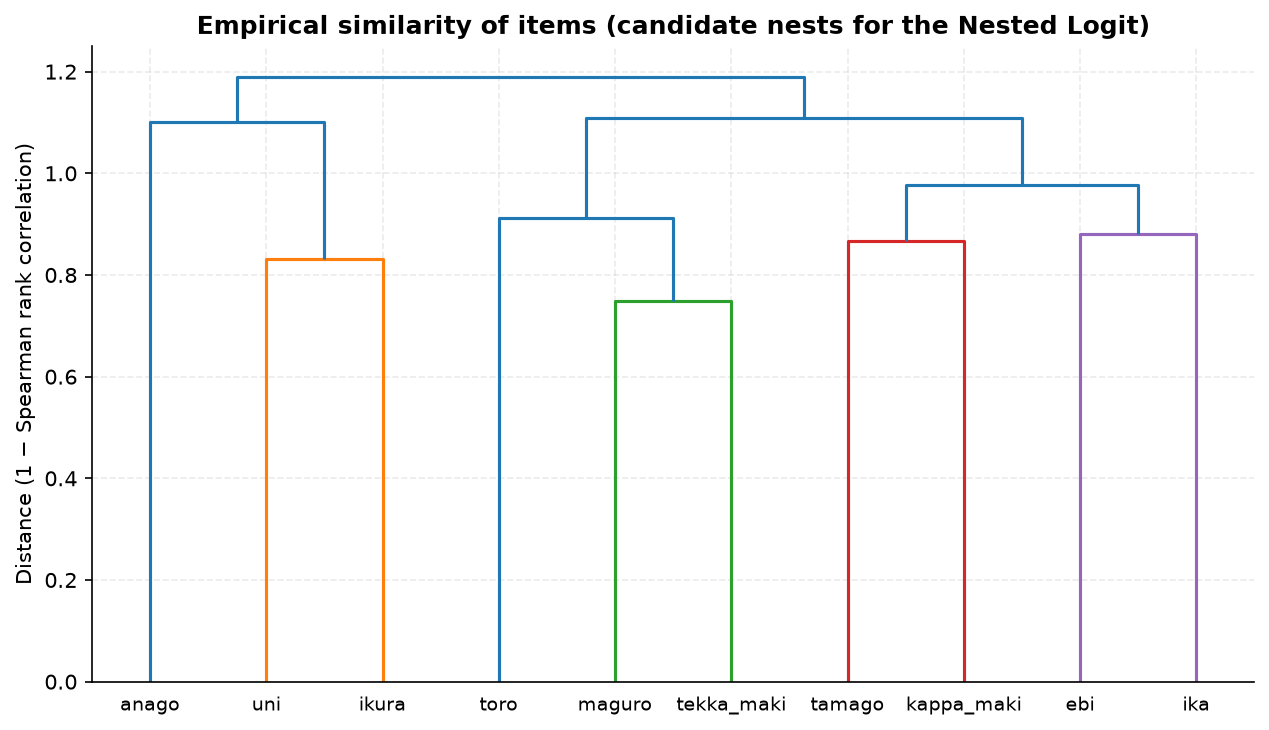
\includegraphics[width=0.55\textwidth]{substitution_dendrogram.png}
  \caption{Clustering jerárquico de ítems según correlación de ranks entre usuarios. El nido \texttt{akami} (maguro, toro, tekka\_maki) emerge empíricamente, validando la estructura de nidos usada en M2.}
  \label{fig:dendro}
\end{figure}

Se definen tres nidos por ingrediente principal (Figura~\ref{fig:dendro}): \textbf{akami} (maguro, toro, tekka\_maki), \textbf{seafood\_other} (ebi, anago, ika, uni, ikura) y \textbf{non\_seafood} (tamago, kappa\_maki). Los parámetros log-sum $\lambda_m \in (0, 1]$ miden la correlación intra-nido: $\lambda_m = 1$ implica MNL dentro del nido; $\lambda_m \to 0$ implica sustitutos perfectos. La estimación se realiza en Apollo (R) con $\lambda_{\text{non\_seafood}}$ fijado en 1 por la razón que se detalla abajo.

\begin{table}[H]
  \centering
  \small
  \caption{M2 --- Nested Logit, ranking explotado ranks 1--3 ($N_{\text{pseudo}} = 15.000$, $K = 11$)}
  \label{tab:m2}
  \begin{tabular}{lrrrr}
    \toprule
    Parámetro & Estimación & EE robusta & $t$ (vs.\ $\lambda=1$) & $p$ \\
    \midrule
    $\lambda_{\text{akami}}$            & 0,323 & 0,027 & $-$26,05 & $< 10^{-3}$ \\
    $\lambda_{\text{seafood\_other}}$   & 0,342 & 0,097 & $-$6,92  & $< 10^{-3}$ \\
    $\lambda_{\text{non\_seafood}}$     & 1,000 & ---   & (fijo)   & --- \\
    \bottomrule
    \addlinespace
    \multicolumn{5}{l}{\footnotesize LL(M2) = $-$29.159,71\;\; LL(MNL-explotado) = $-$29.446,46\;\; LR = 573,5, $\text{gl} = 2$, $p \approx 3 \times 10^{-125}$} \\
    \multicolumn{5}{l}{\footnotesize Los dos $\lambda_m$ libres son $< 1$: IIA se rechaza en akami y seafood\_other.} \\
  \end{tabular}
\end{table}

\textbf{Hallazgo:} IIA se rechaza contundentemente (LR $= 573{,}5$, $p \approx 3 \times 10^{-125}$). El $\lambda_{\text{akami}} = 0{,}323$ implica que maguro, toro y tekka\_maki son sustitutos mucho más cercanos de lo que el MNL predice: cuando el atún favorito no está disponible, el consumidor migra desproporcionadamente hacia otro ítem del mismo nido.

\textbf{Sobre el nido non\_seafood.} Una especificación con los tres $\lambda$ libres empuja $\lambda_{\text{non\_seafood}}$ al límite inferior ($\to 0{,}002$). Esta condición de frontera es un artefacto del nido degenerado (2 ítems con shares 4,1\% y 0,7\%) y no un parámetro de sustitución creíble: en la frontera, tamago y kappa\_maki se comportarían como un solo ítem al filo de la navaja, contaminando las predicciones. Por eso el optimizador de Apollo (BGW) no converge en la variante libre y se fija $\lambda_{\text{non\_seafood}} = 1$ (M2); la variante libre se reporta en la Tabla~\ref{tab:comparison} sólo como referencia de ajuste muestral.

\subsection{M3 --- Modelo de clases latentes}
\label{sec:lc}

Como especificación avanzada con variables latentes se estima un \textit{Latent Class MNL} en Apollo (R) sobre el mismo panel explotado de M2 (3 pseudo-elecciones por usuario; la agrupación panel es la que identifica las clases: los 3 ranks de una persona deben provenir de la misma clase). Cada clase $s$ tiene su propio set completo de ASCs (ebi $= 0$ como referencia dentro de cada clase) y la probabilidad de pertenencia sigue un logit sobre demografía observada:

\begin{equation}
  \pi_{ns} = \frac{\exp(\delta_s + \gamma_{\text{edad},s}\,\text{edad}_n + \gamma_{\text{oeste},s}\,\text{oeste}_n + \gamma_{\text{mujer},s}\,\text{mujer}_n + \gamma_{\text{mig},s}\,\text{mig}_n)}{\sum_{s'}\exp(\cdot)}
  \label{eq:lc}
\end{equation}

Dentro de cada clase las utilidades son ASCs puros: por la restricción de identificación de la Sección~\ref{sec:ident}, betas de atributos específicos por clase serían colineales con los ASCs de la clase. La heterogeneidad se lee en \emph{cómo difieren los ASCs entre clases}. Se estiman especificaciones con $S = 2$ y $S = 3$ clases; la selección usa BIC contra el benchmark de una clase (MNL-explotado):

\begin{table}[H]
  \centering
  \small
  \caption{M3 --- selección del número de clases ($N_{\text{pseudo}} = 15.000$)}
  \label{tab:lc_sel}
  \begin{tabular}{lrrr}
    \toprule
    Modelo & $K$ & LL & BIC \\
    \midrule
    MNL-explotado ($S=1$) & 9  & $-$29.446,5 & 58.979,5 \\
    M3 con $S=2$          & 23 & $-$28.943,0 & 58.107,2 \\
    \textbf{M3 con $S=3$} & \textbf{37} & \textbf{$-$28.513,7} & \textbf{57.383,3} \\
    \bottomrule
    \addlinespace
    \multicolumn{4}{l}{\footnotesize LR $S=3$ vs.\ $S=1$: $1.865{,}4$, gl $= 28$, $p \approx 0$. BIC selecciona \textbf{3 clases}.} \\
  \end{tabular}
\end{table}

\begin{table}[H]
  \centering
  \caption{M3 ($S=3$) --- ASCs por clase (ref.: ebi $=0$) y modelo de membresía}
  \label{tab:lc3}
  \small
  \begin{tabular}{lrrr}
    \toprule
    & Clase a & Clase b & Clase c \\
    Parámetro & \textit{``gourmet premium''} & \textit{``gusto ligero''} & \textit{``fanático del atún''} \\
    \midrule
    \multicolumn{4}{l}{\textit{ASCs por clase (t-ratios entre $|3{,}0|$ y $|21{,}2|$ salvo indicación)}} \\
    ASC$_{\text{anago}}$       &  0,346 & $-$0,380 &  0,302 \\
    ASC$_{\text{maguro}}$      & $-$0,554 & $-$0,576 &  \textbf{1,464} \\
    ASC$_{\text{ika}}$         & $-$0,847 & $-$0,493 & $-$0,494 \\
    ASC$_{\text{uni}}$         &  \textbf{1,850} & $-$2,187 & $-$0,081$^{\dagger}$ \\
    ASC$_{\text{ikura}}$       &  0,917 & $-$0,737 &  0,294 \\
    ASC$_{\text{tamago}}$      & $-$2,176 & $-$0,660 & $-$1,219 \\
    ASC$_{\text{toro}}$        &  1,408 & $-$0,600 &  \textbf{2,838} \\
    ASC$_{\text{tekka\_maki}}$ & $-$2,083 & $-$1,132 &  0,150$^{\dagger}$ \\
    ASC$_{\text{kappa\_maki}}$ & $-$3,366 & $-$1,730 & $-$2,842 \\
    \addlinespace
    \multicolumn{4}{l}{\textit{Membresía (logit multinomial; ref.: clase c)}} \\
    $\delta$ (constante)          & $-$0,630 (t $-$3,9) & $-$0,348 (t $-$2,0) & --- \\
    $\gamma_{\text{edad}}$        &  0,176 (t 3,8)  & $-$0,117 (t $-$2,3) & --- \\
    $\gamma_{\text{oeste}}$       &  0,128 (t 1,2)  &  0,356 (t 3,3)  & --- \\
    $\gamma_{\text{mujer}}$       &  0,384 (t 3,9)  &  0,811 (t 7,9)  & --- \\
    $\gamma_{\text{migró}}$       &  0,037 (t 0,4)  & $-$0,273 (t $-$2,6) & --- \\
    \addlinespace
    \multicolumn{4}{l}{\textit{Perfil posterior de las clases}} \\
    Share de clase       & 33,7\% & 31,3\% & 34,9\% \\
    Grupo etario promedio & 2,13 (el mayor) & 1,76 (el más joven) & 1,97 \\
    \% Japón Occidental  & 30,2\% & 35,7\% & 27,7\% \\
    \% mujeres           & 51,1\% & 64,3\% & 43,4\% \\
    \bottomrule
    \addlinespace
    \multicolumn{4}{l}{\footnotesize $^{\dagger}$ no significativo al 5\%. Fuente: \texttt{latent\_class\_results.csv}, \texttt{latent\_class\_profiles.csv}.} \\
  \end{tabular}
\end{table}

La interpretación conductual de las tres clases se desarrolla en la Sección~\ref{sec:lc_interp}.

\subsection{Comparación de modelos}

\begin{table}[H]
  \centering
  \caption{Comparación de modelos de la cadena de estimación}
  \label{tab:comparison}
  \resizebox{\textwidth}{!}{%
  \begin{tabular}{lrrrrrr}
    \toprule
    Modelo & $N$ & $K$ & LL & $\rho^2$ & AIC & BIC \\
    \midrule
    \multicolumn{7}{l}{\textit{Modelos protagonistas del informe}} \\
    \textbf{M1} (interacciones, Set A)  & \textbf{5.000}  & \textbf{12} & \textbf{$-$9.733,2}  & \textbf{0,155} & \textbf{19.490,4} & \textbf{19.568,6} \\
    \textbf{M2} (Nested Logit, $\lambda_{ns}=1$) & \textbf{15.000} & \textbf{11} & \textbf{$-$29.159,7} & ---            & \textbf{58.341,4} & \textbf{58.425,2} \\
    \textbf{M3} (Latent Class, $S=3$)   & \textbf{15.000} & \textbf{37} & \textbf{$-$28.513,7} & ---            & \textbf{57.101,5} & \textbf{57.383,3} \\
    \midrule
    \multicolumn{7}{l}{\textit{Baselines y variantes (referencia; no discutidos en el cuerpo)}} \\
    MNL-atributos             & 5.000  & 3  & $-$9.850,7  & 0,144 & 19.707,5 & 19.727,0 \\
    MNL-ASC                   & 5.000  & 9  & $-$9.755,1  & 0,153 & 19.528,1 & 19.586,8 \\
    M1r (restringido)         & 5.000  & 10 & $-$9.741,0  & 0,154 & 19.502,0 & 19.567,2 \\
    MNL-explotado             & 15.000 & 9  & $-$29.446,5 & --- & 58.910,9 & 58.979,5 \\
    M2 (variante $\lambda$ libre) & 15.000 & 12 & $-$29.112,1 & ---   & 58.248,3 & 58.339,7 \\
    M3 con $S=2$              & 15.000 & 23 & $-$28.943,0 & ---   & 57.932,0 & 58.107,2 \\
    \bottomrule
  \end{tabular}}
  \\[4pt]
  {\footnotesize LL$_0$ (shares iguales) = $-$11.512,93 en el Set A. Los modelos sobre datos explotados ($N_{\text{pseudo}} = 15.000$) no son comparables en LL con los de primera elección. \textbf{M1} es el preferido para interpretación; \textbf{M2} aporta la sustitución y \textbf{M3} la segmentación.}
\end{table}

\subsection{Validación cruzada Python--Apollo y robustez}
\label{sec:robust}

\begin{enumerate}[nosep]
  \item \textbf{Validación cruzada con Apollo (R).} Los modelos se re-estimaron en Apollo 0.3.7 como motor de máxima verosimilitud independiente de la implementación propia en Python/scipy. Las log-verosimilitudes coinciden: M1 ($-$9.733,207 vs.\ $-$9.733,21; $\Delta$ = 0,004) y M2 ($-$29.159,71, $\Delta$ = 0,01); los coeficientes coinciden a 4 decimales. El M3 (Latent Class) se estimó directamente en Apollo y se verificó reconstruyendo su verosimilitud de forma manual e independiente en \texttt{04\_lc\_postprocess.R}: la LL reconstruida coincide con la de Apollo al centésimo ($-$28.513,74). Los baselines también se replicaron con $\Delta \leq 0{,}001$, garantizando que los tests LR no dependen del software.
  \item \textbf{Exclusión de los autores del dataset}: los usuarios 323, 617, 1431 y 4667 son los autores del paper (Kamishima, 2003). Re-estimar M1 sin ellos cambia los coeficientes en a lo más $|\Delta\beta| = 0{,}003$: despreciable.
  \item \textbf{Estabilidad de ranks}: los ASCs estimados sólo con la primera elección vs.\ con ranks 1--3 explotados difieren hasta en 6 errores estándar para maguro y tekka\_maki (que funcionan como ``segunda opción'' sistemática) y para uni (que polariza: se ama o se odia). Esta deriva es una limitación declarada de la explosión de rankings (Sección~\ref{sec:limit}) y, a la vez, evidencia de heterogeneidad de gustos ---la motivación del modelo de clases latentes (Sección~\ref{sec:lc}).
\end{enumerate}

% =============================================================================
\section{Parameter Interpretation and Behavioral Insights (Sección B)}
\label{sec:B}
% =============================================================================

\subsection{El precio como señal de calidad}
\label{sec:price_quality}

El baseline MNL-atributos entrega $\beta_{\text{precio}} = +0{,}581$ ($z = 24{,}1$), positivo y altamente significativo. En un contexto de elección convencional donde el consumidor paga, $\beta_{\text{precio}}$ sería negativo (mayor precio $\rightarrow$ menor utilidad). Aquí el signo opuesto surge porque se trata de una encuesta de ranking de preferencias sin restricción presupuestaria: el consumidor expresa \emph{preferencia}, no \emph{compra}. Los ítems más caros (toro en 4,49; uni en 3,29) son también los más preferidos, de modo que el precio opera como \emph{señal de calidad} y no como costo.

Las consecuencias operativas son:
\begin{itemize}[nosep]
  \item Los ratios WTP calculados por método delta no son interpretables como disposición a pagar monetaria. Se reportan sólo como trade-offs relativos (Apéndice~\ref{app:wtp}).
  \item Los escenarios contrafactuales de precio deben interpretarse con cautela: en este modelo un \emph{aumento} de precio eleva la utilidad (señala mayor calidad), lo contrario de la intuición económica estándar. Además, la $\text{corr}(\text{precio},\text{oiliness}) = 0{,}82$ infla el error estándar de $\beta_{\text{precio}}$, por lo que su magnitud exacta debe tomarse con cautela.
\end{itemize}

\subsection{Edad y preferencia por la grasa}
\label{sec:age_oil}

La interacción $\beta_{\text{oil}\times\text{edad}} = +0{,}089$ de M1 ($z = 5{,}2$, $p < 10^{-6}$) es uno de los hallazgos más sólidos del informe. Los consumidores japoneses de mayor edad derivan sistemáticamente más utilidad del sushi grasoso, incluso después de controlar por la preferencia promedio de cada ítem (capturada en los ASCs).

\begin{figure}[H]
  \centering
  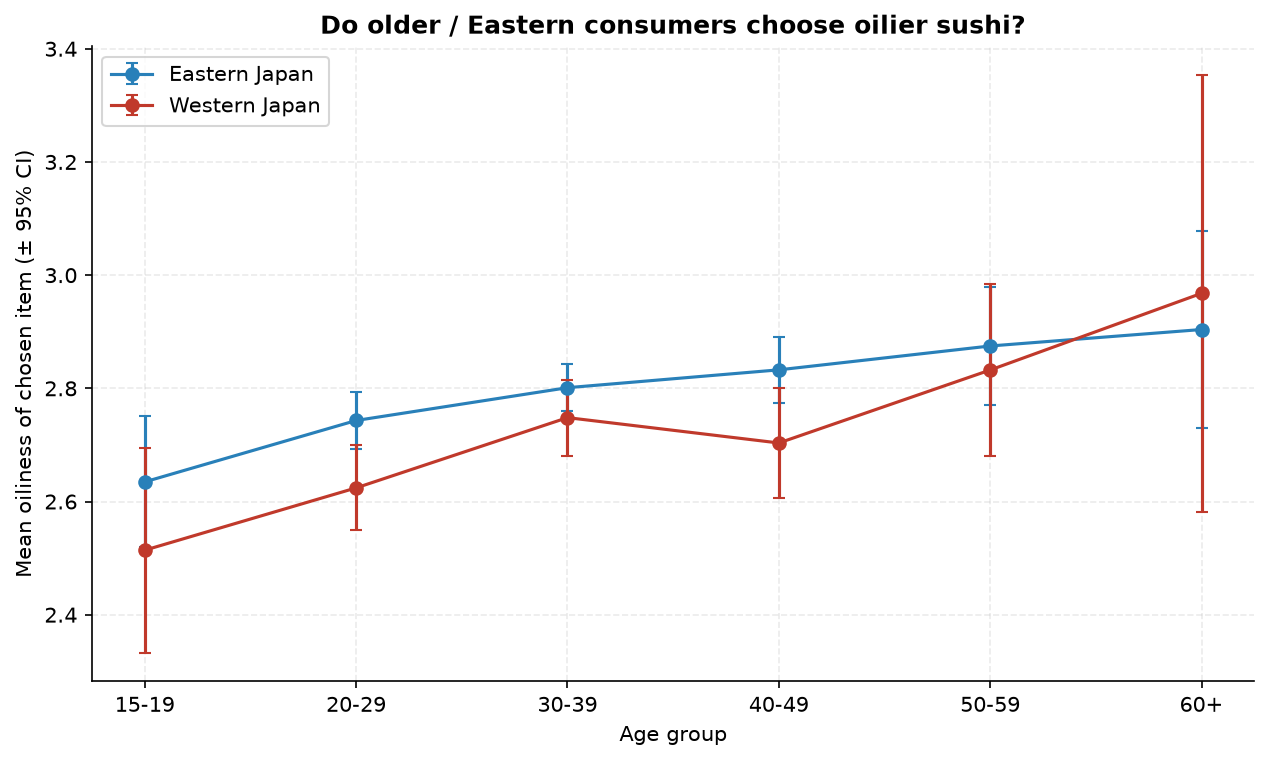
\includegraphics[width=0.62\textwidth]{oiliness_by_eastwest.png}
  \caption{Oiliness promedio del ítem elegido, por grupo etario y región Este/Oeste. Los consumidores mayores del Japón Oriental eligen los ítems más grasosos (toro, anago), consistente con la interacción $\beta_{\text{oil}\times\text{edad}}$ significativa.}
  \label{fig:oil_age}
\end{figure}

El resultado es coherente con la cultura gastronómica japonesa: el sushi tradicional ``Edo-mae'' (estilo Tokio) enfatiza cortes grasos e intensos, y la preferencia por estos sabores se intensifica con la edad y la experiencia culinaria.

\subsection{Heterogeneidad regional Este--Oeste}

Japón exhibe una división culinaria Este--Oeste documentada (el propio README del dataset la describe). M1 incluye dos interacciones con Oeste, ambas de $|z| < 1{,}96$ individualmente:
\begin{itemize}[nosep]
  \item $\beta_{\text{precio}\times\text{oeste}} = -0{,}066$ ($z = -1{,}46$): evidencia débil de mayor sensibilidad al precio en el Oeste.
  \item $\beta_{\text{oil}\times\text{oeste}} = -0{,}058$ ($z = -0{,}86$): evidencia débil de preferencia por sushi menos grasoso en el Oeste.
\end{itemize}

Sin embargo, la Figura~\ref{fig:eastwest} muestra diferencias Este--Oeste sistemáticas en los shares, y el test LR conjunto es significativo: $\text{LR} = 15{,}6$, $\text{gl} = 2$, $p = 4{,}1 \times 10^{-4}$. La debilidad individual se atribuye a la $\text{corr}(\text{precio}, \text{oiliness}) = 0{,}82$: el modelo no logra separar si la aversión occidental es al precio o a la grasa cuando ambos atributos se mueven juntos.

\begin{figure}[H]
  \centering
  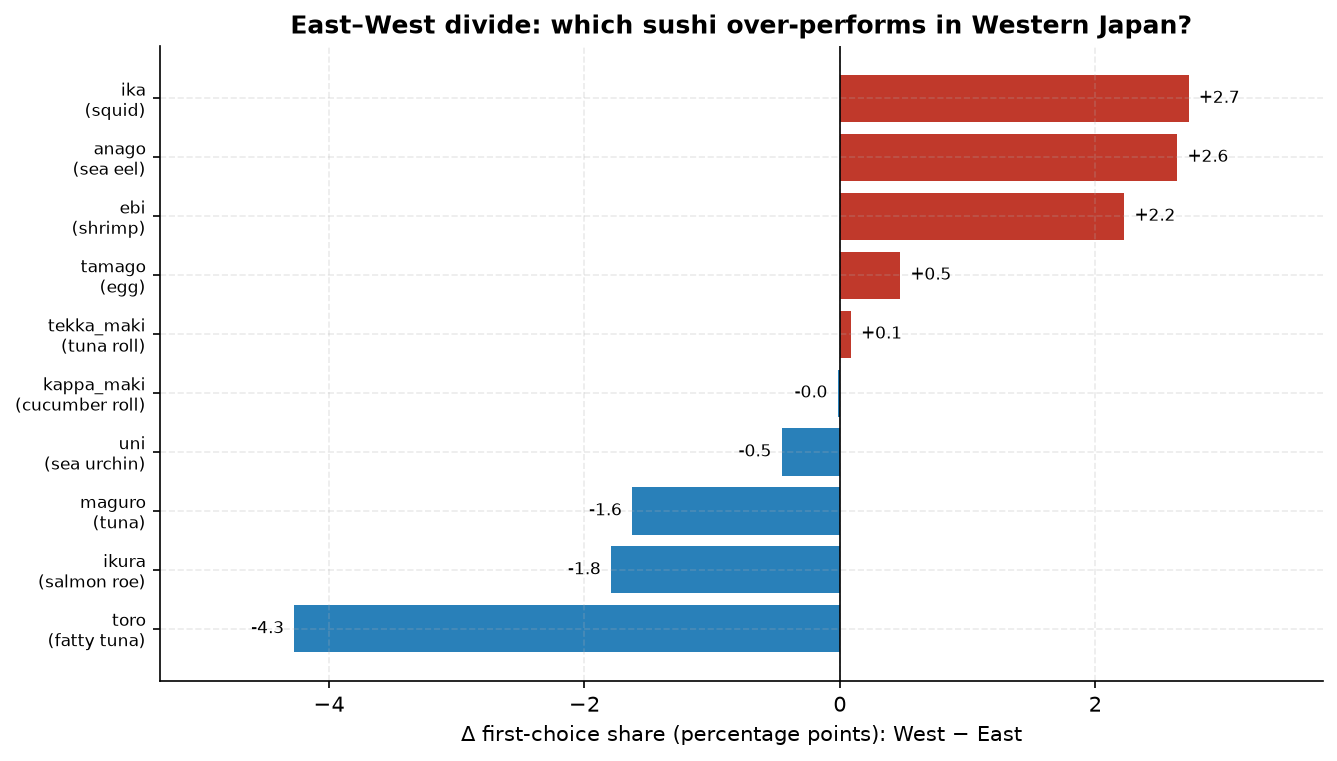
\includegraphics[width=0.62\textwidth]{eastwest_preferences.png}
  \caption{Diferencia de shares de primera preferencia entre Japón Occidental y Oriental, por ítem. Los ítems ligeros (ika, anago, ebi) sobre-rinden en el Oeste; toro e ikura, en el Este.}
  \label{fig:eastwest}
\end{figure}

\subsection{Patrones de sustitución: IIA rechazado}

El Nested Logit M2 entrega la evidencia más fuerte contra el supuesto IIA:
\begin{itemize}[nosep]
  \item $\lambda_{\text{akami}} = 0{,}323$: maguro, toro y tekka\_maki son sustitutos \emph{tres veces más cercanos} de lo que el MNL predice. Si toro no está disponible, el consumidor migra desproporcionadamente a maguro y tekka\_maki y no hacia mariscos de otros nidos.
  \item $\lambda_{\text{seafood\_other}} = 0{,}342$: correlación intra-nido similar para el grupo amplio de productos del mar.
  \item $\lambda_{\text{non\_seafood}} = 1$ (fijo): el nido degenerado (tamago y kappa\_maki) se trata como MNL dentro del nido para evitar la frontera $\lambda \to 0$ (ver Sección~\ref{sec:m2}).
\end{itemize}
El dendrograma de clustering jerárquico (Figura~\ref{fig:dendro}) valida la estructura de nidos de forma independiente: la distancia de correlación de ranks entre maguro, toro y tekka\_maki es mucho menor que entre cualquiera de ellos y los ítems de otros nidos.

\subsection{Segmentos latentes de consumidores}
\label{sec:lc_interp}

El modelo de clases latentes M3 (Tabla~\ref{tab:lc3}) segmenta el mercado en tres tipos de consumidor de tamaños casi iguales:
\begin{itemize}[nosep]
  \item \textbf{Clase a --- ``gourmet premium'' (33,7\%).} Prefiere los mariscos intensos y caros: uni ($+1{,}85$, el ASC más alto de la clase), toro ($+1{,}41$) e ikura ($+0{,}92$); rechaza fuertemente huevo y rolls ($-2{,}1$ a $-3{,}4$). Es la clase de mayor edad (grupo etario promedio 2,13) y su membresía crece con la edad ($\gamma_{\text{edad}} = +0{,}18$, $t = 3{,}8$): la versión ``entre personas'' del hallazgo $\beta_{\text{oil}\times\text{edad}}$ de M1.
  \item \textbf{Clase b --- ``gusto ligero'' (31,3\%).} Todos los ASCs son negativos: su ítem favorito es la referencia \emph{ebi} (camarón), y su mayor rechazo es justamente uni ($-2{,}19$), el favorito de la clase a. Es la clase más joven (1,76), más occidental (35,7\%; $\gamma_{\text{oeste}} = +0{,}36$, $t = 3{,}3$) y marcadamente femenina (64,3\%; $\gamma_{\text{mujer}} = +0{,}81$, $t = 7{,}9$).
  \item \textbf{Clase c --- ``fanático del atún'' (34,9\%).} Concentra su preferencia en el nido akami completo: toro ($+2{,}84$), maguro ($+1{,}46$) y tekka\_maki (único segmento donde el rollo de atún tiene ASC positivo). Es la clase más masculina (43,4\% mujeres) y más oriental (27,7\% Oeste).
\end{itemize}

Tres convergencias refuerzan la validez del análisis. La clase c es la contraparte ``entre personas'' del nido akami del NL: la sustitución intra-atún de M2 ($\lambda_{\text{akami}} = 0{,}323$) y la existencia de un segmento atún-céntrico son dos manifestaciones del mismo fenómeno. La polarización de uni detectada en el chequeo de estabilidad de ranks queda explicada: uni es el favorito de la clase a ($+1{,}85$) y el más rechazado de la clase b ($-2{,}19$). Y el gradiente etario y regional de la membresía replica las interacciones de M1 con una lectura más accionable: los tres segmentos son direccionables por edad, género y región observables.

\subsection{Limitaciones}
\label{sec:limit}

\begin{enumerate}[nosep]
  \item \textbf{Preferencia declarada, no revelada}: los rankings expresan preferencia, no compra efectiva bajo restricción presupuestaria. El coeficiente de precio positivo es esperable en este contexto, pero limita la validez externa de los escenarios de precio.
  \item \textbf{Multicolinealidad en el Set A}: $\text{corr}(\text{precio}, \text{oiliness}) = 0{,}82$ infla los errores estándar e impide separar limpiamente los canales de precio y grasa; por eso los escenarios de precio se interpretan cualitativamente.
  \item \textbf{Supuesto de la explosión de rankings}: el exploded logit asume estabilidad de preferencias entre etapas del ranking. El chequeo de estabilidad revela derivas no triviales para maguro y uni.
  \item \textbf{Choice set fijo}: los 5.000 usuarios evalúan los mismos 10 ítems. Esto habilita tests LR potentes pero limita la generalización a ítems fuera del Set A.
  \item \textbf{WTP no monetario}: todas las estimaciones de disposición a pagar están en unidades de precio normalizado, no en JPY; sólo valen para comparaciones relativas entre atributos.
\end{enumerate}

% =============================================================================
\section{Scenario Analysis and Prediction (Sección C)}
\label{sec:C}
% =============================================================================

Se simulan dos escenarios contrafactuales sobre el Set A usando constantes calibradas y los betas de atributo del baseline MNL-atributos (metodología en la Sección~\ref{sec:ident}).

\subsection{Escenario A --- Shock de oferta del toro (+40\% precio)}

\textbf{Intervención}: el precio normalizado del toro aumenta 40\%, simulando una reducción de cuotas de pesca de atún rojo. Se contrasta MNL (constantes calibradas + $\beta$ de MNL-atributos) vs.\ Nested Logit con los $\lambda$ de \textbf{M2} ($\lambda_{\text{akami}} = 0{,}323$, $\lambda_{\text{seafood\_other}} = 0{,}342$, $\lambda_{\text{non\_seafood}} = 1$).

\begin{figure}[H]
  \centering
  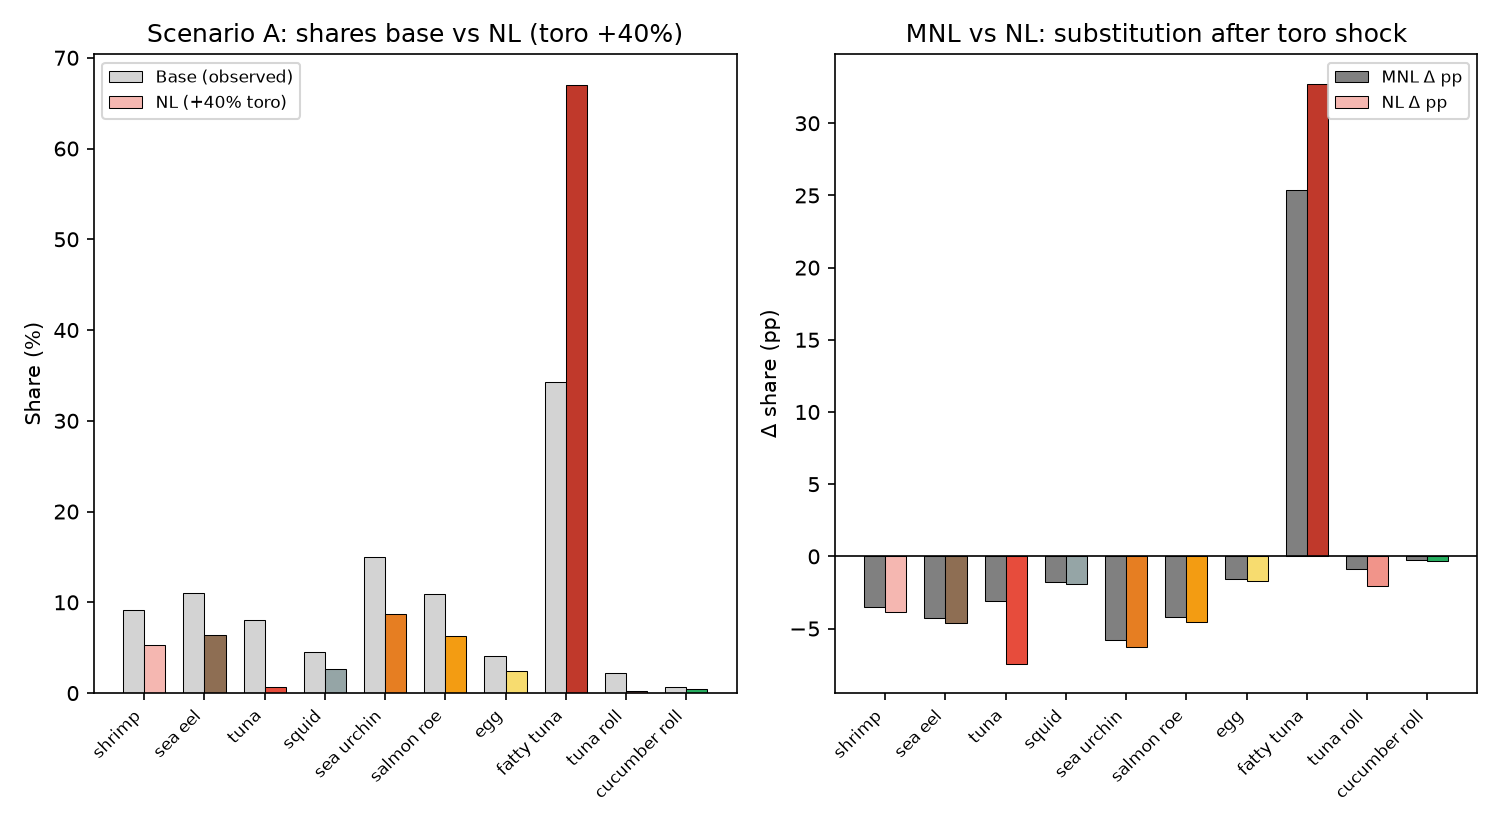
\includegraphics[width=0.92\textwidth]{scenario_A_nl_mnl.png}
  \caption{Escenario A: shares y $\Delta$ (pp) tras el shock de +40\% en el precio del toro, comparando MNL y NL. El NL predice que los ítems del mismo nido (maguro, tekka\_maki) pierden \emph{más} share que bajo MNL: consecuencia de $\lambda_{\text{akami}} = 0{,}323$.}
  \label{fig:scenarioA}
\end{figure}

\begin{table}[H]
  \centering
  \small
  \caption{Escenario A --- shock del toro: shares y elasticidades}
  \label{tab:scenarioA}
  \begin{tabular}{lrrrc}
    \toprule
    Ítem & Base \% & MNL \% & NL \% & Elasticidad cruzada (MNL) \\
    \midrule
    Toro (atún graso)     & 34,3 & 59,7 & 67,0 & 1,853 (propia) \\
    Maguro (atún)         &  8,1 &  5,0 &  0,6 & $-$0,966 \\
    Anago (anguila)       & 11,0 &  6,8 &  6,4 & $-$0,966 \\
    Uni (erizo)           & 14,9 &  9,2 &  8,7 & $-$0,966 \\
    Ikura (huevas salmón) & 10,9 &  6,7 &  6,3 & $-$0,966 \\
    Ebi (camarón)         &  9,2 &  5,6 &  5,3 & $-$0,966 \\
    Ika (calamar)         &  4,6 &  2,8 &  2,7 & $-$0,966 \\
    Tamago (huevo)        &  4,1 &  2,5 &  2,4 & $-$0,966 \\
    Tekka-maki (rollo atún)& 2,3 &  1,4 &  0,2 & $-$0,966 \\
    Kappa-maki (pepino)   &  0,7 &  0,4 &  0,4 & $-$0,966 \\
    \bottomrule
  \end{tabular}
  \\[4pt]
  {\footnotesize Todas las elasticidades cruzadas MNL son idénticas ($-$0,966): firma del IIA; las del NL difieren por nido. \textbf{Caveat}: $\beta_{\text{precio}} > 0 \rightarrow$ el alza de precio eleva la utilidad (señal de calidad; ver Sección~\ref{sec:price_quality}).}
\end{table}

\textbf{Hallazgo clave}: bajo MNL todas las elasticidades cruzadas son idénticas ($-$0,966), la firma del IIA. Bajo NL, los ítems del nido akami se canibalizan mucho más de lo que el MNL predice: maguro cae 7,5 pp (frente a 3,1 pp bajo MNL) y tekka\_maki 2,1 pp (frente a 0,9 pp), porque $\lambda_{\text{akami}} = 0{,}323$ implica sustitución cercana dentro del nido del atún. Esta respuesta diferencial es el insight central: la escasez de toro desplaza la demanda desproporcionadamente hacia los otros formatos de atún, un patrón invisible para el MNL. (La magnitud del alza de toro depende del $\beta_{\text{precio}}$ inflado por multicolinealidad; el resultado robusto es el \emph{patrón} de sustitución MNL vs.\ NL, no la cifra exacta.)

\subsection{Escenario B --- Promoción saludable (kappa-maki)}

\textbf{Intervención}: kappa-maki (rollo de pepino) recibe una reducción de precio de 30\% junto a una campaña de visibilidad que eleva su \texttt{freq\_sold} de 0,40 al percentil 75 (0,88). Los betas de atributo provienen de MNL-atributos con constantes calibradas; la heterogeneidad se modela con las interacciones de M1 por edad y región Este/Oeste.

\begin{figure}[H]
  \centering
  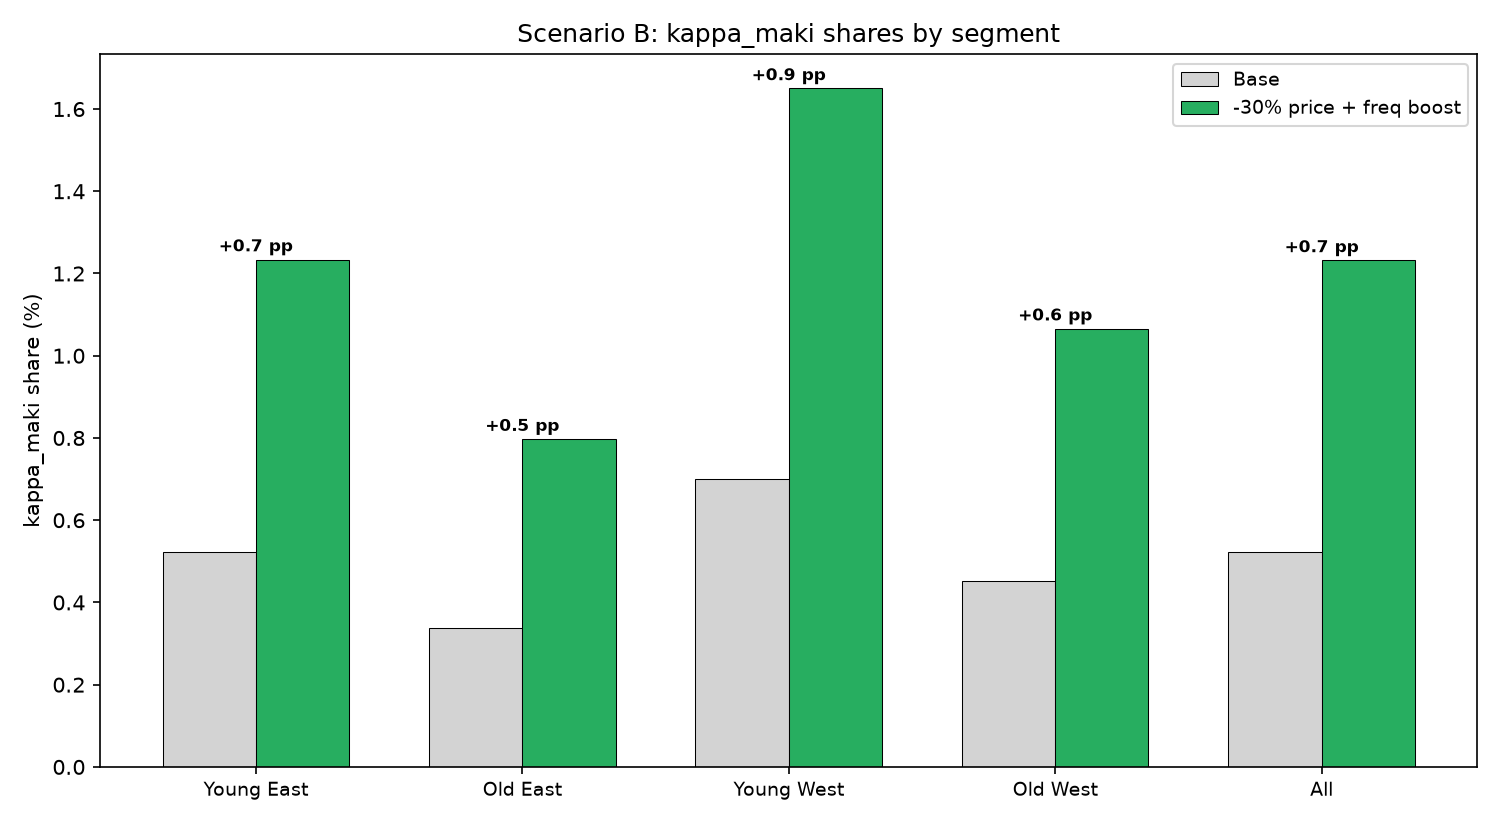
\includegraphics[width=0.82\textwidth]{scenario_B_segments.png}
  \caption{Escenario B: shares predichos de kappa-maki por segmento demográfico, base vs.\ contrafactual.}
  \label{fig:scenarioB}
\end{figure}

\begin{table}[H]
  \centering
  \small
  \caption{Escenario B --- share de kappa-maki por segmento}
  \label{tab:scenarioB}
  \begin{tabular}{lrrcc}
    \toprule
    Segmento & $n$ & Base \% & CF \% & $\Delta$ (pp) \\
    \midrule
    Joven Este  & 2.515 & 0,523 & 1,234 & +0,711 \\
    Mayor Este  &   933 & 0,337 & 0,797 & +0,460 \\
    Joven Oeste & 1.126 & 0,701 & 1,650 & +0,949 \\
    Mayor Oeste &   426 & 0,451 & 1,066 & +0,614 \\
    \textbf{Total} & \textbf{5.000} & \textbf{0,522} & \textbf{1,232} & \textbf{+0,709} \\
    \bottomrule
  \end{tabular}
  \\[4pt]
  {\footnotesize La ganancia de share la domina el aumento de \texttt{freq\_sold} ($\beta_{\text{freq}} = +2{,}17$); la rebaja de 30\% en el precio \emph{reduce} utilidad porque $\beta_{\text{precio}} > 0$, así que el efecto neto viene de la disponibilidad.}
\end{table}

\textbf{Hallazgo clave}: el share de kappa-maki pasa de 0,52\% a 1,23\% (+0,71 pp), una ganancia modesta en términos absolutos pero que más que duplica el share base, impulsada casi por completo por el aumento de \texttt{freq\_sold} ($\beta_{\text{freq}} = +2{,}17$); la rebaja de precio opera en dirección contraria porque $\beta_{\text{precio}} > 0$. Los jóvenes occidentales muestran la mayor respuesta (+0,95 pp), consistente con el hallazgo de M1 de que el Oeste interactúa negativamente con la grasa: kappa-maki es el ítem menos grasoso del Set A.

% =============================================================================
\section{Strategic and Public Policy Recommendations (Sección D)}
\label{sec:D}
% =============================================================================

\subsection{Para cadenas de restaurantes y retail de sushi}

\textbf{Diseño de menú informado por sustitución.} El hallazgo del Nested Logit M2 ($\lambda_{\text{akami}} = 0{,}323$) tiene implicancias directas para inventario y menú:
\begin{itemize}[nosep]
  \item Cuando el toro se agota, la demanda \emph{no} se reparte uniformemente por el menú: se concentra en maguro y tekka\_maki, los ítems de su mismo nido. Un restaurante que anticipe escasez de toro debe reforzar el stock de maguro y tekka\_maki, no reponer proporcionalmente.
  \item El nido non\_seafood (tamago y kappa\_maki) funciona como un único bloque funcional. Agregar una tercera opción sin pescado probablemente canibalice a estas dos en vez de expandir el mercado.
\end{itemize}

\textbf{Segmentación etaria y regional.} Los hallazgos de M1 y del modelo de clases latentes M3 (Secciones~\ref{sec:age_oil} y~\ref{sec:lc_interp}) indican que las campañas de ítems premium grasos (toro, anago, uni) deben dirigirse a consumidores mayores del Japón Oriental (el segmento ``gourmet premium'' / ``fanático del atún''), mientras que los ítems ligeros y vegetales (kappa\_maki, tamago) resuenan más con el segmento ``gusto ligero'': jóvenes, occidentales y mayoritariamente mujeres. Los tres segmentos son direccionables con variables observables (edad, género, región).

\subsection{Para la política de salud pública}

\textbf{Las campañas de alimentación saludable basadas en precio difícilmente funcionarán} en el mercado del sushi. El escenario de kappa-maki (Sección~\ref{sec:C}) muestra que incluso con una rebaja de 30\% y un fuerte impulso de disponibilidad, el share del ítem más saludable del Set A sube sólo de 0,52\% a 1,23\%: una ganancia pequeña en términos absolutos y dominada por el aumento de disponibilidad más que por la rebaja de precio.

Más importante: $\beta_{\text{precio}} > 0$ implica que el consumidor japonés usa el precio como heurística de calidad. Un ``sushi saludable'' subsidiado se percibiría como de \emph{menor calidad}, socavando la intervención. Las campañas deberían usar palancas distintas del precio:
\begin{itemize}[nosep]
  \item \textbf{Disponibilidad y visibilidad}: $\beta_{\text{freq\_sold}} = +2{,}17$ (el mayor coeficiente de atributo) sugiere que aumentar la presencia de opciones saludables en menús y tiendas tiene un efecto real y cuantificable.
  \item \textbf{Educación y framing}: en vez de bajar el precio, reposicionar los estilos ligeros como elecciones premium de artesanía culinaria, no como ``alternativas saludables baratas''.
\end{itemize}

\subsection{Recomendaciones metodológicas para trabajo futuro}

\begin{enumerate}[nosep]
  \item \textbf{Datos de preferencia revelada}: transacciones reales con precios pagados resolverían el confounding $\beta_{\text{precio}} > 0$ y harían interpretables el WTP y los escenarios de precio en términos monetarios.
  \item \textbf{Variación de atributos a nivel individual}: si los consumidores enfrentaran precios o composiciones distintas (p.\,ej.\ vía diseño experimental), betas de atributos y ASCs serían identificables conjuntamente sin calibración, resolviendo también la multicolinealidad precio-grasa.
  \item \textbf{Mixed Logit}: una especificación con coeficientes aleatorios continuos complementaría al modelo de clases latentes para capturar la heterogeneidad residual dentro de clase (la deriva de ranks de uni y maguro).
\end{enumerate}

\newpage
\section*{Bibliografía}
\addcontentsline{toc}{section}{Bibliografía}

\begin{enumerate}[nosep,leftmargin=*]
  \item Beggs, S., Cardell, S., \& Hausman, J. (1981). Assessing the potential demand for electric cars. \textit{Journal of Econometrics}, 17(1), 1--19.
  \item Hess, S. \& Palma, D. (2019). Apollo: A flexible, powerful and customisable freeware package for choice model estimation. \textit{Journal of Choice Modelling}, 32, 100170.
  \item Kamishima, T. (2003). Nantonac Collaborative Filtering: Recommendation Based on Order Responses. \textit{Proceedings of KDD2003}, 583--588.
  \item Train, K. (2009). \textit{Discrete Choice Methods with Simulation} (2.ª ed.). Cambridge University Press.
\end{enumerate}

\section*{Linkografía}
\addcontentsline{toc}{section}{Linkografía}

\begin{itemize}[nosep,leftmargin=*]
  \item Dataset original: \url{https://www.kamishima.net/sushi/}
  \item Carpeta compartida con datos y scripts:\\[2pt]
        \fbox{\parbox{0.9\linewidth}{\centering\textbf{PENDIENTE: insertar link (Drive/GitHub) antes de entregar}}}
\end{itemize}

\newpage
\appendix
\section{Apéndice: trade-offs relativos entre atributos}
\label{app:wtp}

\begin{table}[H]
  \centering
  \small
  \caption{Trade-offs relativos calculados desde MNL-atributos (no son WTP monetario; ver Sección~\ref{sec:price_quality})}
  \label{tab:wtp}
  \begin{tabular}{lccc}
    \toprule
    Trade-off & Estimación & EE & IC 95\% \\
    \midrule
    Oiliness / Precio    & $-$0,147 & 0,067 & [$-$0,278; $-$0,016] \\
    Freq\_sold / Precio  & $-$3,739 & 0,278 & [$-$4,283; $-$3,195] \\
    \bottomrule
    \addlinespace
    \multicolumn{4}{l}{\footnotesize Método delta sobre $-\beta_k/\beta_{\text{precio}}$ (baseline MNL-atributos, Set A, $N = 5.000$).} \\
    \multicolumn{4}{l}{\footnotesize Con $\beta_{\text{precio}} > 0$ el ratio no es disposición a pagar monetaria; sólo trade-off relativo.} \\
  \end{tabular}
\end{table}

\section{Apéndice: modelos del informe y nombres en el código}
\label{app:map}

Los nombres de modelo del informe se corresponden con los siguientes nombres internos de los scripts (columna \texttt{model} de los CSV en \texttt{outputs/tables/}):

\begin{table}[H]
  \centering
  \small
  \begin{tabular}{lll}
    \toprule
    Nombre en el informe & Nombre en el script & Fuente \\
    \midrule
    M1 (preferido, interacciones)  & \texttt{M3\_interactions} & \texttt{02\_estimate\_models.py} \\
    M2 (Nested Logit)              & \texttt{M4b}              & \texttt{03\_exploded\_models.py} / Apollo \\
    M3 (Latent Class, $S=3$)       & \texttt{LC3}              & \texttt{03\_apollo\_latent\_class.R} \\
    MNL-atributos                  & \texttt{M1\_attributes}   & \texttt{02\_estimate\_models.py} \\
    MNL-ASC                        & \texttt{M2\_asc}          & \texttt{02\_estimate\_models.py} \\
    MNL-explotado                  & \texttt{M2exp}            & \texttt{03\_exploded\_models.py} \\
    M1r (restringido)              & \texttt{M3r\_restricted}  & \texttt{02\_estimate\_models.py} \\
    M2 (variante $\lambda$ libre)  & \texttt{M4}               & \texttt{03\_exploded\_models.py} \\
    M3 con $S=2$                   & \texttt{LC2}              & \texttt{03\_apollo\_latent\_class.R} \\
    \bottomrule
  \end{tabular}
\end{table}

\begin{verbatim}
scripts/
  config.py                Configuracion central
  process_sushi_dataset.py Pipeline raw -> CSV (mapeo Set A corregido)
  verify_sushi_dataset.py  47 checks de integridad de datos
  01_eda_visualizations.py 11 figuras + 5 tablas resumen
  02_estimate_models.py    Baselines + M1 (scipy BFGS, grad. analitico)
  03_exploded_models.py    M2 Nested Logit (ranking explotado)
  04_scenario_analysis.py  2 escenarios contrafactuales (A toro, B kappa)
R_Studio/
  apollo_config.R          Configuracion Apollo
  apollo_data_prep.R       Pivot long -> wide + explosion de ranks
  01_apollo_mnl.R          Baselines + M1 (validacion cruzada)
  02_apollo_nested_logit.R MNL-explotado y M2 (validacion cruzada)
  03_apollo_latent_class.R M3: clases latentes (2 y 3 clases)
  04_lc_postprocess.R      Shares y perfiles posteriores del LC
  EXPLICACION_MODELOS_R.txt Guia de cada modelo R y sus conclusiones
\end{verbatim}

Todos los scripts Python son reproducibles (SEED = 42). Los scripts de Apollo se ejecutaron con R 4.5.3 y Apollo 0.3.7; sus salidas (\texttt{APOLLO\_*\_output.txt}, \texttt{*\_estimates.csv}) quedan en \texttt{outputs/tables/} como evidencia de ejecución.

\end{document}
